\documentclass[11pt,a4paper]{article}
\usepackage[latin1]{inputenc}
\usepackage{amsmath}
\usepackage{graphicx}
\usepackage{amsfonts}
\usepackage{amssymb}
\title{Challenges of the analysis of large graphs}
\author{Luc Hogie, Frédéric Giroire, Stéphane Perennes, Thibaud Trolliet}
\begin{document}
\maketitle


This paper describes JMaxGraph, a Java library for the analysis of large graph topologies.





The objective of this paper is to describe our experience in dealing with
a large dataset representing the connections between users in Twitter. It enumerates the obstacles we faced, and exposes the solutions we had
to find for each of them in order to reach our goal.

\paragraph{The dataset}
{
The Twitter datasets was collected by the DIANA research group (Inria) in 2011. It is single 215GB text file. 
398,846,191 vertices, 23,137,510,395 arcs
This file stores a graph made of 400M arcs and 23G vertices. 
}

\paragraph{Our objective}
{
Our objective was to compute the number of occurrences of certain topological patterns in this graph.
}




\section{State of the Art}

There exist numerous libraries for graph manipulation, like JGraphT, Jung, LEDA, Jung, etc. These libraries cannot be used when the garph is


Our attempts to manipulate the graph with common graph libraries failed because  of both the memory and computational overhead of the data-structures they employ.
JGraphT enables the

Distributed graph platforms such as Hadoop Giraph and Spark GraphX boast the ability to deal with very large graphs.  The solve the inherent complexity of distributed computing by proposing the BSP programming model. BSP is a vertex-centric message-based programming model which is very adequate to the implementation of simple vertex-centric algorithms. Unfortunately it cannot be used for algorithms that have no natural vertex-centric expression, for which it imposes poor performance because of network congestion due to too numerous messages transiting.
Even though we succeeded in implementing algorithms in those platforms, GraphX cannot be used because of its huge memory requirements and unreliable behavior.

\section{Objectives}




\section{Loading the graph}


The Twitter graph initially came as an ADJ file. The ADJ file format defines that the first line of the file is the number of vertices. Each following line then consists of:
\begin{enumerate}
\item the ID of the vertex;
\item the number of neighbors;
\item the ID for each neighbor.
\end{enumerate}
Numbers are separated by a space.


Using 16MB buffer.
The read throughput of the cluster is 600MB/s. Transferring the entire file to RAM takes 6mn.

Using Java standard buffering I/O and number parsing, loading the entire graph takes min. The read throughput then MB/s.

1
2
4
8		4.5=>2.5
16
32

We profiled the execution and we discovered that both  the  basic I/O primitives for reading data from the file and the number parsing methods dramatically slowed down the process. By analyzing the source code of the Java standard library, we found out that the responsible is the excessive number of method calls. These methods had not been in-lined by the just-in-time compiler.

We made a new implementation of buffered reading and number parsing, which speeds up the graph loading process by a factor 30, as illustrated on Figure \ref{fig-a}. Thereby reducing the loading time to 7min. We can see that the graph loading speed is very close to the speed of pure data transfer to memory, which means that the time spent turning text data to graph data-structure is insignificant. Thus at this point, the bottleneck becomes the disk reads. This motivated the definition of a the JMG file format.


\begin{figure}
\begin{center}
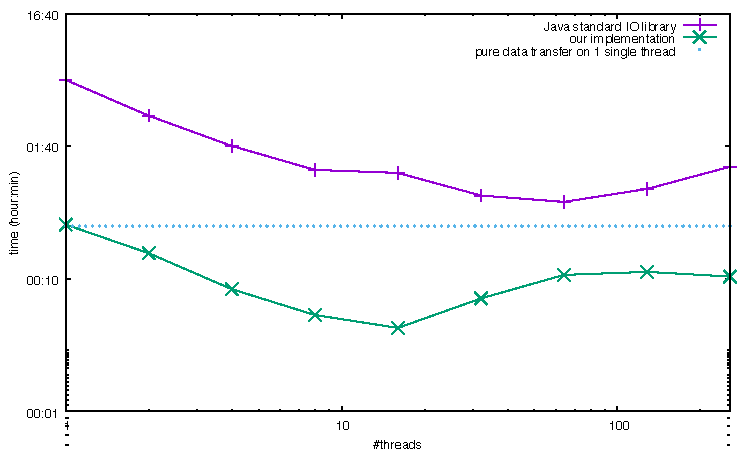
\includegraphics[width=0.8\linewidth]{load.pdf}
\end{center}
\caption{blabla}
\end{figure}


\subsection{The JMG file format}
In the JMG format, the graph is described by several files in a directory. Two file types:

The \texttt{properties.txt}  is an ASCII text file. It consists of a sequence of $key=value$ lines. It stores various graph property, such as the number of vertices in the graph.

ARC files store adjacencies. A JMG directory embeds at least one ARC file, which stores either the OUT-adj or the IN-adj. But it may contain the ARC files for both directions.
The IN (resp. OUT) adjacency is expected to be found in a file \texttt{in.arc} (resp. \texttt{out.arc}). Such ARC file comes with its index file, called \texttt{-index.nbs}. An NBS file is a binary fixed-length encoding for integer numbers.
For each vertex $u$, the index file has an entry which gives the position in the adjacency file at which the set of neighbors of $u$ are stored.

In the ARC file, this set of neighbors is encoded at a byte sequence of length:
$$l = index(u+1) - index(u)$$
 Note that if $u$ is the vertex with the highest ID,  they does not exist such thing as $index(u+1))$. The length of the byte sequence describing its neighborhoods is then defined by:
 $$l = size(indexFile) - index(u)$$
Note also that the number neighbors cannot be computed out of this $l$, as every vertex may use words of different length to store their neighborhood.
Then, starting at position $index(u)$, the byte sequence encoding the set of neighbors for vertex $u$ is organized like this:
\begin{enumerate}
\item 8 bytes encode the neighbor with lowest ID
\item 1 byte encodes the number of bytes used to store each other neighbor, let us refer to it as $e$. The number of neighbors is then defined by $1 + \frac{l - 9}{e}$.
\item each following neighbor $v_i$ of $u$ is encoded as the delta $d$ of its ID and the ID of the previous neighbor.
The ID of the $i^{th} (with\ i > 0)$ neighbor is obtained by:
$$v_i = v_{i-1} + d$$.
\end{enumerate}

The JMG file format exhibits the following advantages:
\begin{enumerate}
\item adjacency lists are ordered, which is very profitable to algorithms which can hence resort to dichotomy.
\item the dataset can be accessed randomly. This means that the degree and the adjacency of any given vertex can be retrieved from disk without having to load/parse other vertices.
\item an ARC file is iterable. This means that adj-list contains in an ARC file can be processed on-the-fly when the file is loaded. This mechanism fastens algorithms which process any adj-list one single time and make it possible to execute certain algorithms even though there is not enough RAM to load the entire graph.
\item there is no vertex in adjacency lists that is not in the vertex set.
\item adjacency lists are compressed in such a way that the more an adj-list is long, the fewer bytes will be used to store each individual element.
\item compression/decompression time is insignificant
\end{enumerate}

The Twitter datasets is 3-times smaller when encoded as a JMG datasets rather than stored in an ADJ file.

\section{Data structure}

Need to support memory and disk operations
The vertex space is contiguous. Vertices ID range from 0 to N-1, N being the number of vertices in the graph.


\subsection{On minimizing RAM usage}

In the Hotspot JVM, object overhead is 8 bytes. Moreover every object occupies a number of bytes that is a multiple of 8. If the number of bytes required by an object for its header and fields is not a multiple 8, then you round up to the next multiple of 8.  

As a consequence, an instance of a Vertex class with one single int field to store the ID of the vertex requires occupies 16 bytes. Each reference to this instance uses 8 more bytes (in a 64bit memory model). Note that if an object is not referenced, it is destroyed by the garbage collector. The vertex set of the Twitter graph is 9.6GB. The adj-list occupies 184GB.


\subsection{int[][]}

The adj-list are stored in an array. Neighbors of vertex $u$ can in found at the $u^{th}$ cell, referred to as $adj[u]$.
Adj-list are ordered. The $u^{th}$ neighbor of vertex $u$ can be obtained by $adj[u][i]$.

\section{Graph processing}
\subsection{Multi-threading}

\subsection{BSP}


\subsection{Map/Reduce}
inherently
incremental
resilient to failures
distributed, with no restriction whatsoever on the number of workers which can be changed at any time

\section{Algorithms}



\section{Additional features}

Progress monitoring



\end{document}